In this section we provide the whole \texttt{Alloy} code used for the analysis of the \hyperref[tab:acronymsTable]{S2B}, the results of the assertions and the diagrams representing the different worlds generated by the predicates.

\subsection{Alloy Code}
\alloyfile{Alloy/alloy code.als}

\newpage


\subsection{Assertions}

\begin{figure}[H]
    \centering
    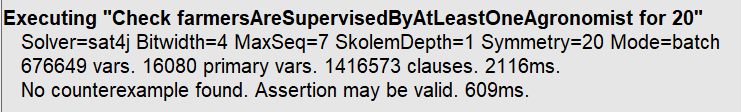
\includegraphics[]{Images/Alloy/assertion - farmersAreSupervisedByAtLeastOneAgronomist.png}
    \caption{Assertion 1}
    \label{fig:assertion1}
\end{figure}

\begin{figure}[H]
    \centering
    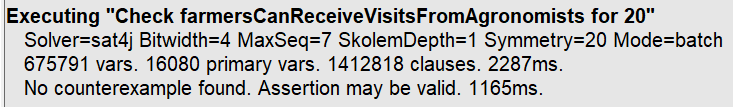
\includegraphics[]{Images/Alloy/assertion - farmersCanReceiveVisitsFromAgronomists.png}
    \caption{Assertion 2}
    \label{fig:assertion2}
\end{figure}

\begin{figure}[H]
    \centering
    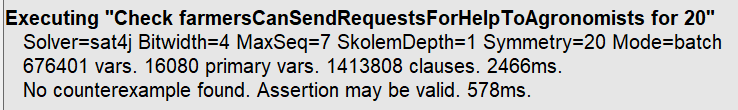
\includegraphics[]{Images/Alloy/assertion - farmersCanSendRequestsForHelpToAgronomists.png}
    \caption{Assertion 3}
    \label{fig:assertion3}
\end{figure}

\begin{figure}[H]
    \centering
    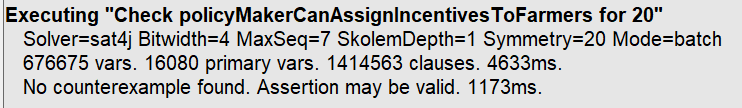
\includegraphics[]{Images/Alloy/assertion - policyMakerCanAssignIncentivesToFarmers.png}
    \caption{Assertion 4}
    \label{fig:assertion4}
\end{figure}

\newpage

\subsection{Worlds}

In this section we present the world diagrams generated by the Alloy predicates. This worlds are intended to show separate parts of the system, each one focusing on a different aspect.

\subsubsection*{World 1}
Figure \ref{fig:world1} represents a world focused on Daily Plans and Visits. It is possible to see that visits belonging to a specific daily plan have the same date of that daily plan. Also, a farmer cannot be visited twice in the same daily plan, while it is possible to receive visits in separate days. Moreover, it is possible to see that the farmers and the agronomist belong to the same area. In the end, each user has its own credentials.

\subsubsection*{World 2}
Figure \ref{fig:world2} represents a world focused on Requests, in this case a request for help. It is possible to see that each message sent in the "chat" is received by all the participants (except the sender, of course), while those users who do not belong to the "chat" (in this case Farmer1) cannot send or receive messages of that conversation. Also, a request has at least one agronomist as a participant (in this case even two). Moreover, the first message of the "chat" (ChatMessage2, isRequestMessage = True) is correctly sent by the farmer that made the request (Farmer0, startingUser), while the other messages are replies. In the end, each user has its own credentials.

\subsubsection*{World 3}
Figure \ref{fig:world3} represents a world focused on Forums. It is possible to see that different farmers can write (send a message) in the forum and each message is received by all farmers, while the agronomist does not participate to the forum. As for Requests (world 2), also here there is the correct mapping between the startingMessage (DiscussionMessage3) and the startingUser (Farmer0). In the end, each user has its own credentials.

\subsubsection*{World 4}
Figure \ref{fig:world4} represents a world focused on Good Practices. It is possible to see that each good practice has been requested by a policy maker and requested to a good-performing farmer. Also, the content of each practice is out of the scope of the analysis and is collapsed to a single entity (Text). Moreover, the agronomist does not act directly in this process. In the end, each user has its own credentials.

\subsubsection*{World 5}
Figure \ref{fig:world5} represents a world focused on Incentives. It is possible to see that a policy maker can assign incentives to a farmer (in this case different incentives to the same farmer) and there can be incentives not assigned yet (Incentive2). In this situation there are also two areas: each area has at least one agronomist (in this case the same one) and each farmer belongs to only one area. In the end, each user has its own credentials.

\newpage

\begin{figure}[H]
    \centering
    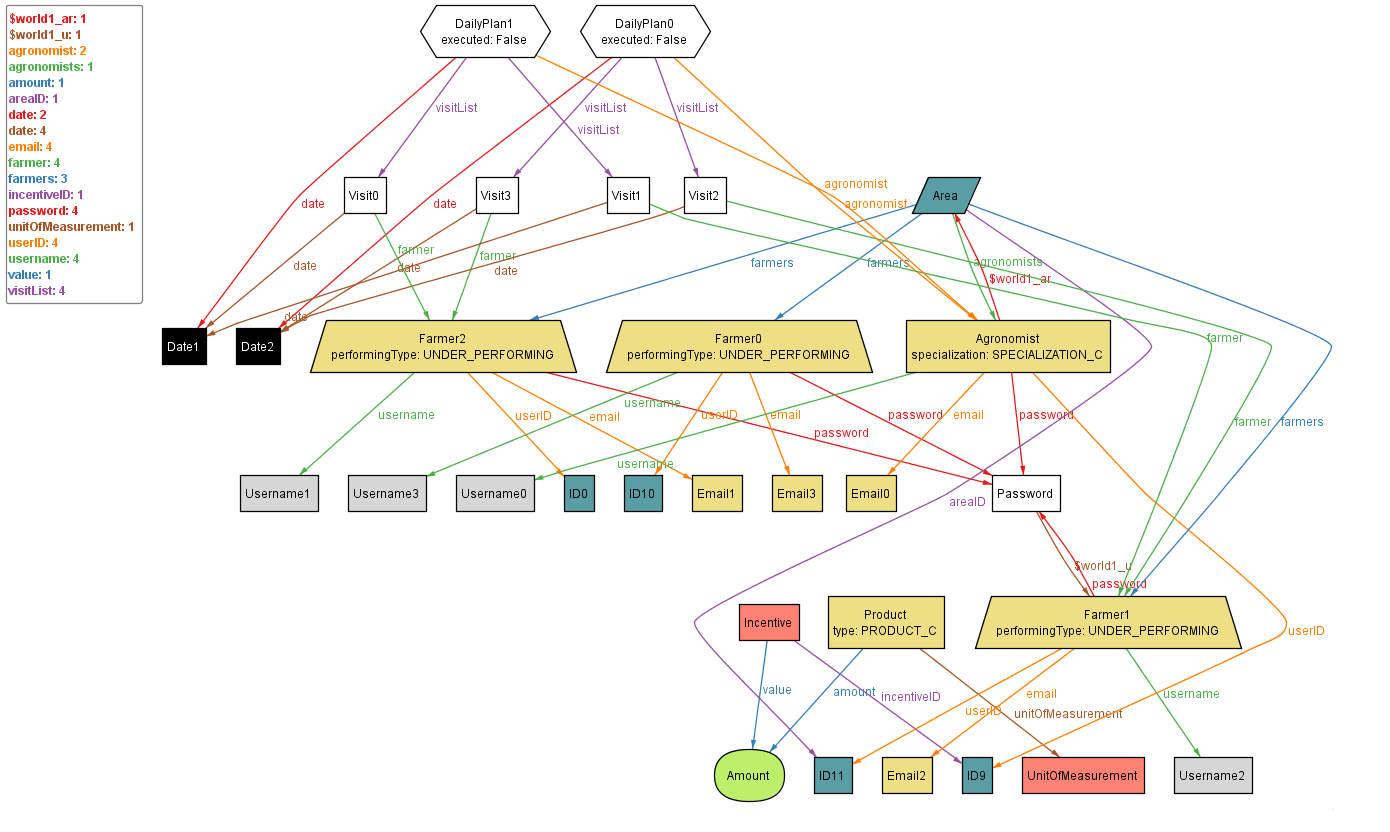
\includegraphics[angle=90, origin=c, width=0.85\textwidth]{Images/Alloy/world1.png}
    \caption{World focused on Daily Plans and Visits}
    \label{fig:world1}
\end{figure}

\begin{figure}[H]
    \centering
    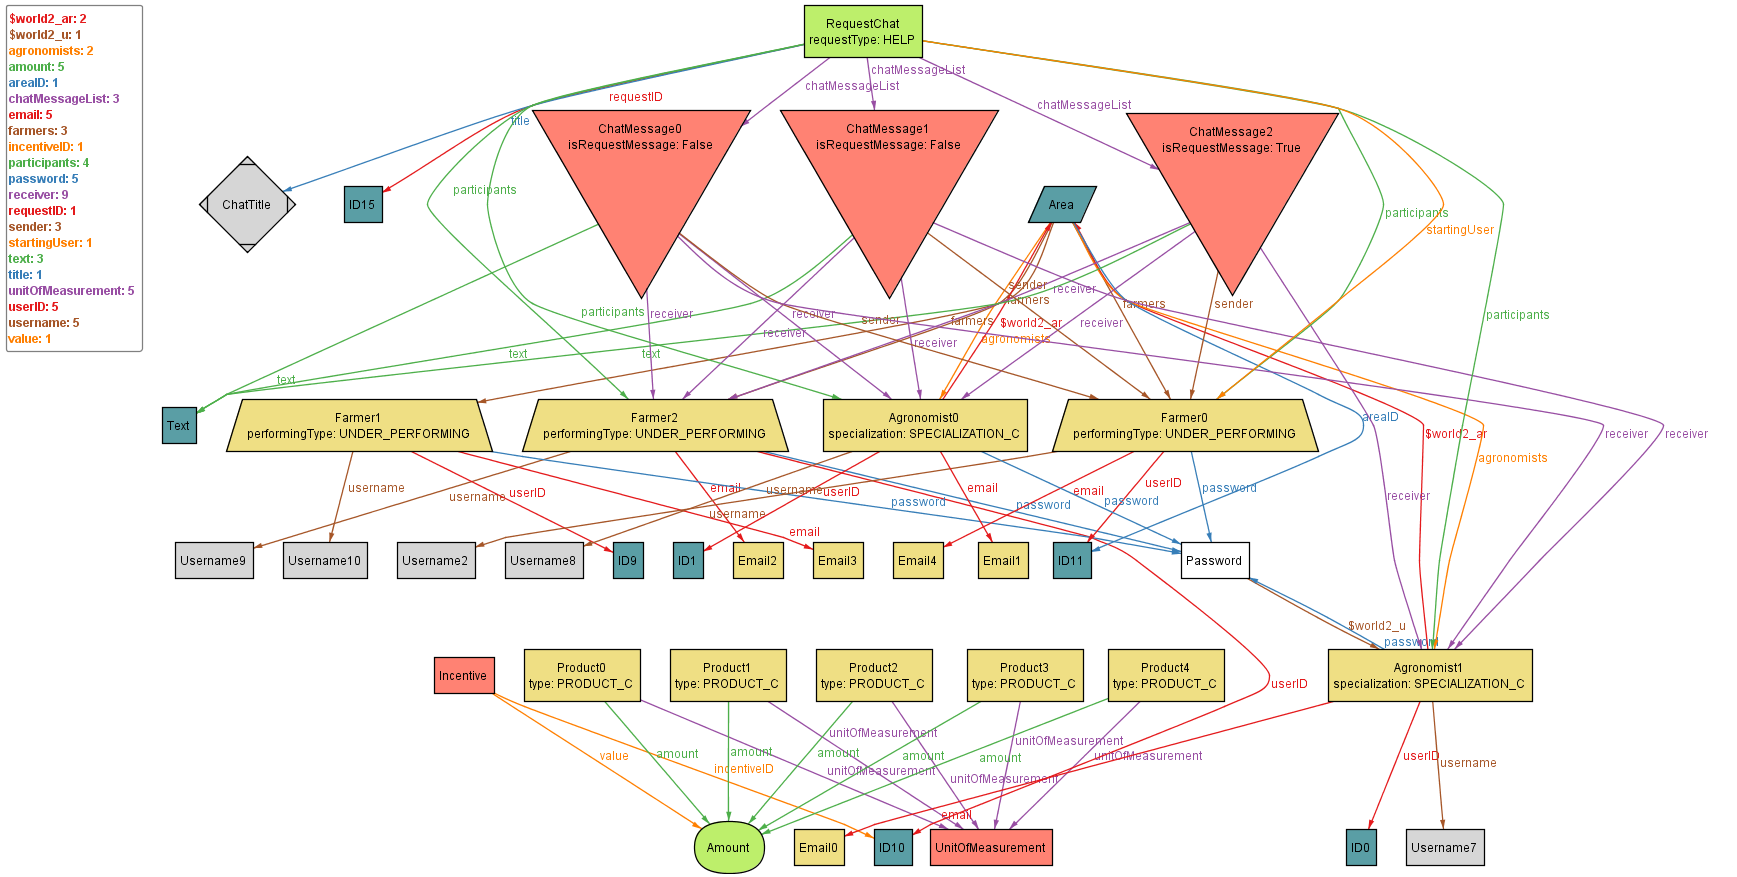
\includegraphics[angle=90, origin=c, width=0.75\textwidth]{Images/Alloy/world2.png}
    \caption{World focused on Requests}
    \label{fig:world2}
\end{figure}

\begin{figure}[H]
    \centering
    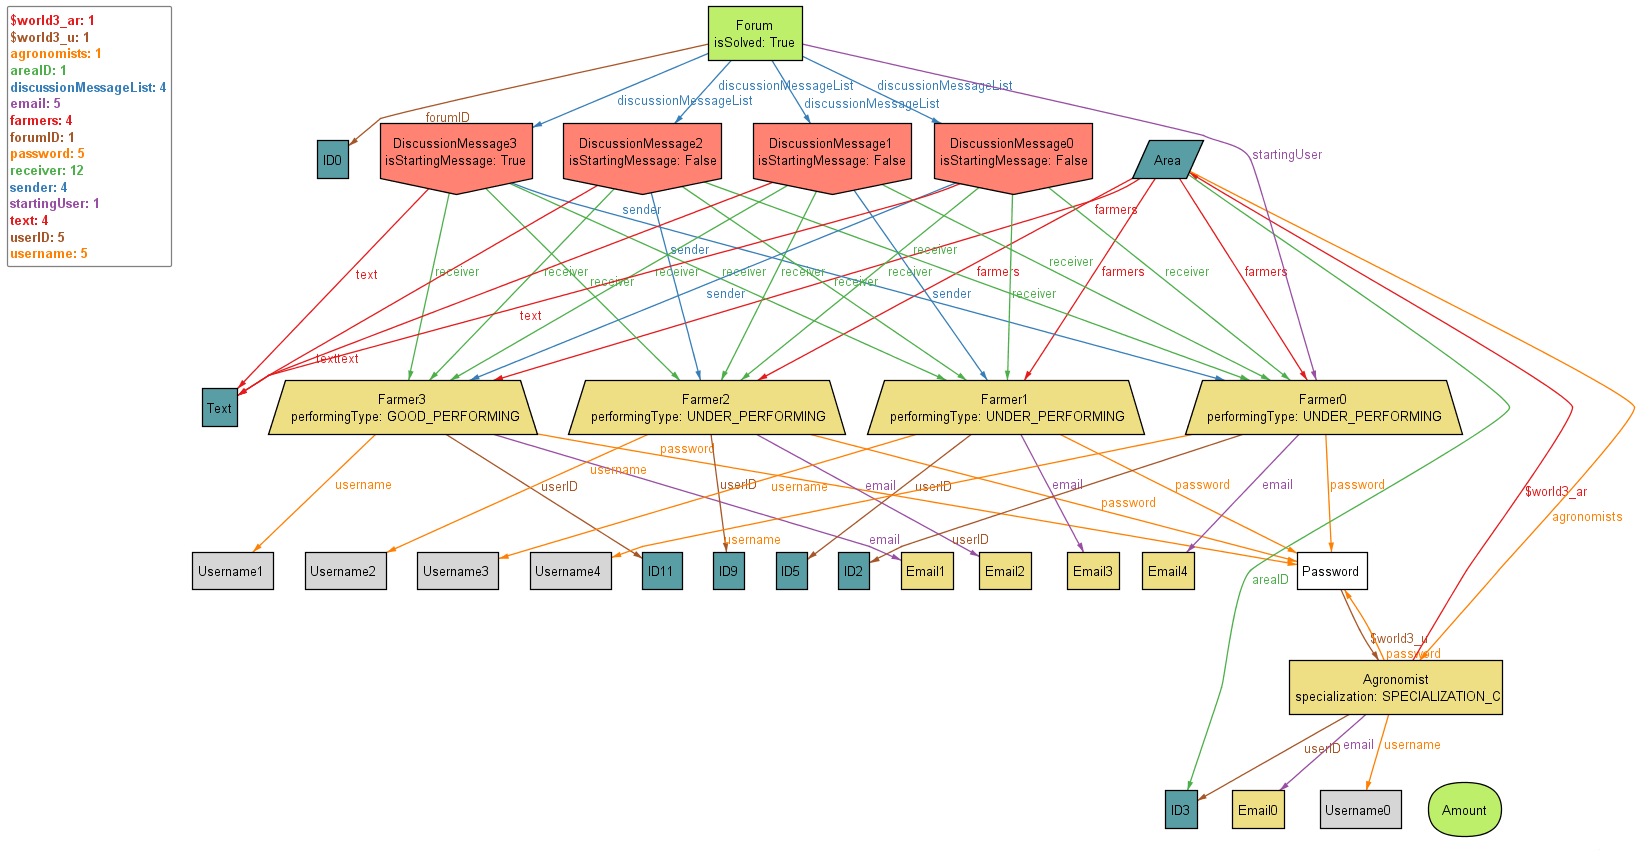
\includegraphics[angle=90, origin=c, width=0.75\textwidth]{Images/Alloy/world3.png}
    \caption{World focused on Forums}
    \label{fig:world3}
\end{figure}

\begin{figure}[H]
    \centering
    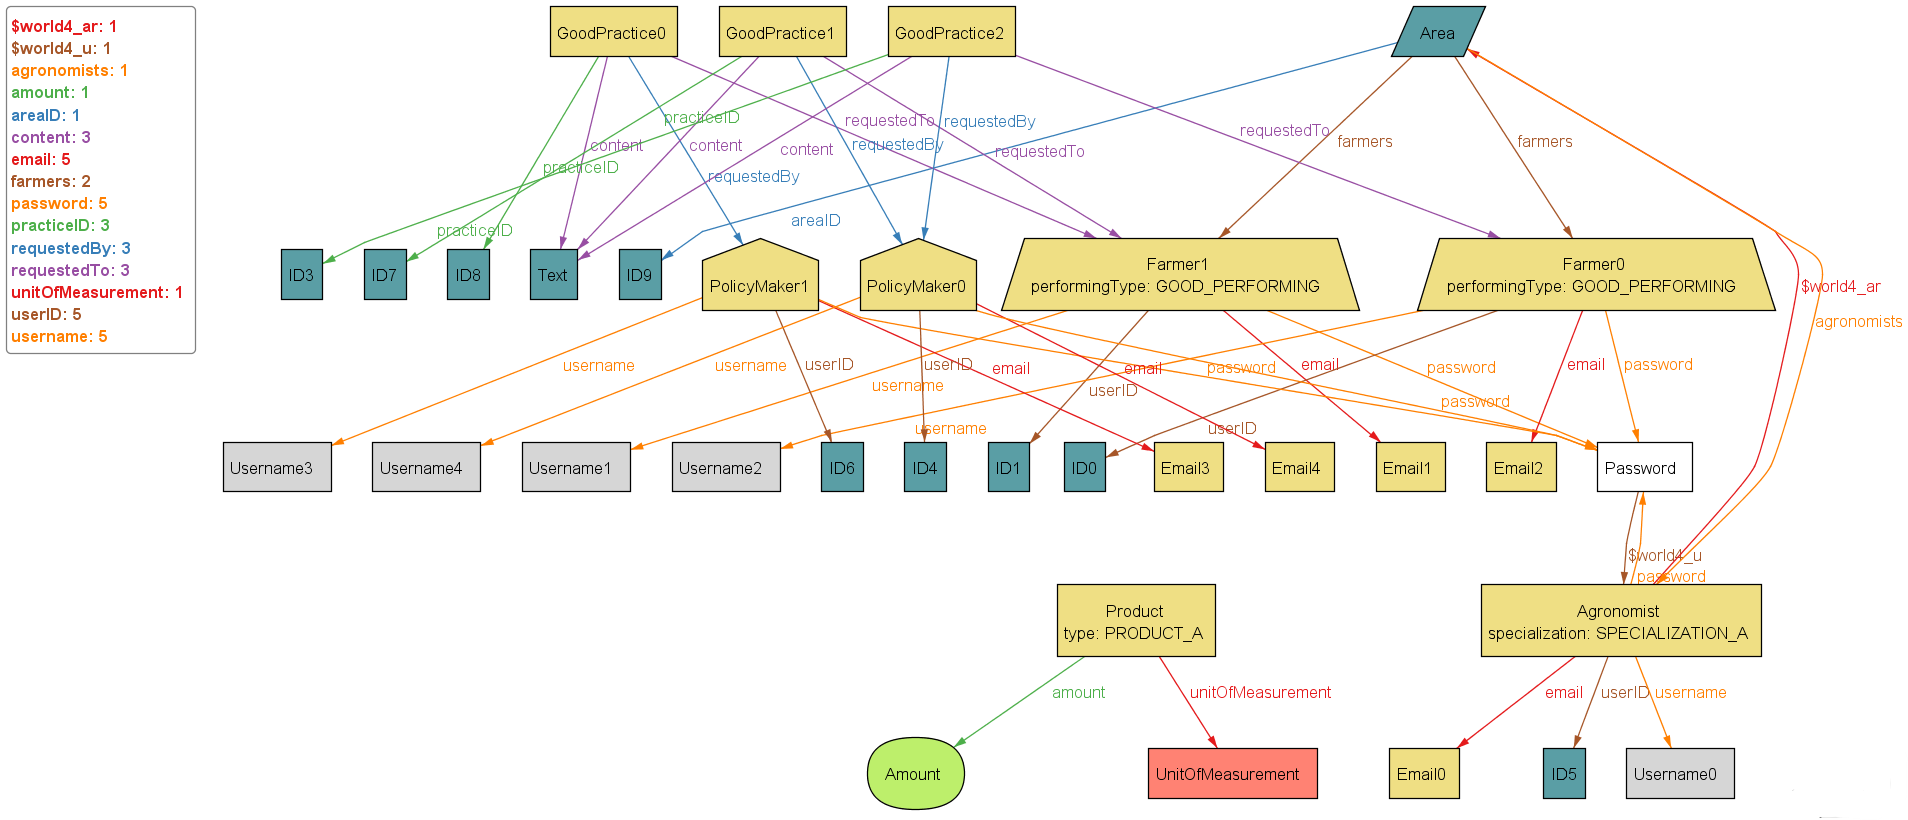
\includegraphics[angle=90, origin=c, width=0.6\textwidth]{Images/Alloy/world4.png}
    \caption{World focused on Good Practices}
    \label{fig:world4}
\end{figure}

\begin{figure}[H]
    \centering
    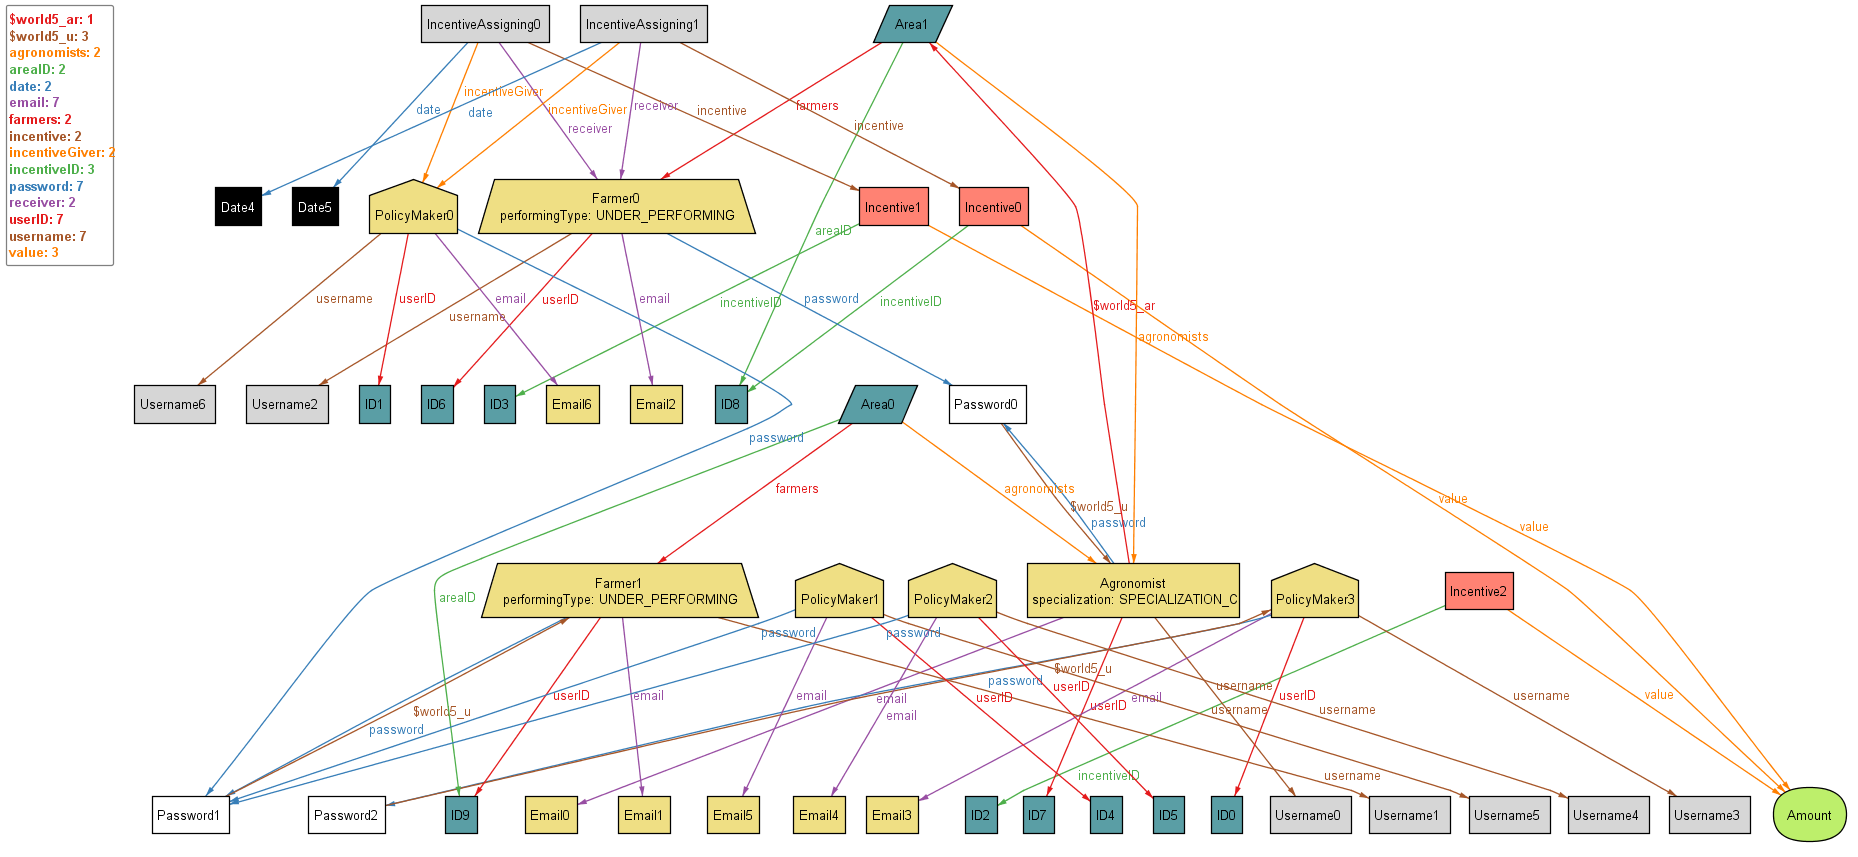
\includegraphics[angle=90, origin=c, width=0.65\textwidth]{Images/Alloy/world5.png}
    \caption{World focused on Incentives}
    \label{fig:world5}
\end{figure}